\chapter{算法测试}
\par 为了测试算法的正确性,需要用尽可能全面的数据样例来测试。根据算法构成,设计了数据对数据处理算法模块、路径求解算法模块以及整体算法进行测试。障碍物数据分为输入的原始数据,以底面平行边的两中点$M_0,M_1$、底面边长D和z轴范围$z_0,z_1$给出,格式为[$M_0$, $M_1$], D, [$z_0$, $z_1$];处理后的障碍物数据为离散到指定精度后的底面四顶点A、B、C、D的坐标以及z轴范围,格式为[A, B, C, D], [$Z_0$, $Z_1$]。效果显示使用Matlab绘制出障碍物与起点到终点所经过的路径,可以直观的看出算法寻路效果 \cite{r7}。

\section{数据处理算法测试}
\par 对数据处理模块而言,算法代码主要是代码\ref{code:obstacle_vertice_process},即将输出的数据信息格式化到可以供后续算法使用的格式,主要是关于计算障碍物底部四个顶点和将顶点离散到指定精度下。测试数据如表\ref{tab:process_input_test_data1}。
\begin{table}[htb]
    \centering
    \caption{输入测试数据1}
    \label{tab:process_input_test_data1}
    \begin{tabular}{cccc}
        \toprule
        起点&终点&障碍物&精度\\
        \midrule
        (0, 0, 0)&(5, 5, 5)&(0.5, 0.5), (3.7, 3.7), 1, [0.2, 4]&0.1\\
        \bottomrule
    \end{tabular}
\end{table}
测试数据为起点终点经过了单个障碍物的情况,此时障碍物信息如表\ref{tab:process_input_test_data1_obstacle1}。障碍物底面是由中点为(0.5, 0.3),(3.7, 3.7),边长为1的矩形组成,高度z轴范围为[0.2, 4]。
\begin{table}[htb]
    \centering
    \caption{障碍物1信息}
    \label{tab:process_input_test_data1_obstacle1}
    \begin{tabular}{ccc}
        \toprule
        底面平行边的两中点&底面边长&z轴范围\\
        \midrule
        (0.5, 0.5) (3.7, 3.7)&1&[0.2, 4]\\
        \bottomrule
    \end{tabular}
\end{table}
根据算法\ref{code:obstacle_vertice_process},计算出障碍物的数据为四顶点的坐标分别为(0.146447, 0.853553), (3.34645, 4.05355), (4.05355, 3.34645), (0.853553, 0.146447),此时,使用Matlab绘制出关于此障碍物的图像,图像如图\ref{fig:obstacle_ex_bottom}。
\begin{figure}[htb]
    \centering
    \caption{数据处理测试障碍物底面}
    \label{fig:obstacle_ex_bottom}
    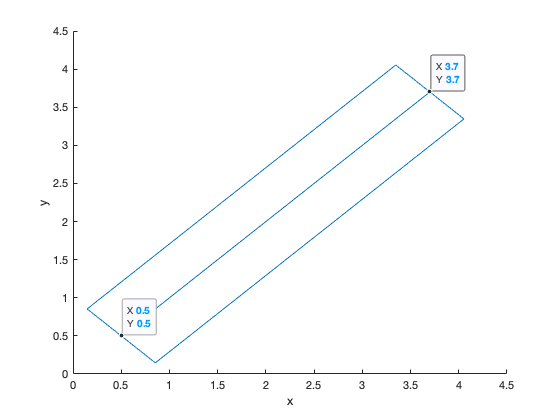
\includegraphics[width=10cm]{figures/obstacle_ex_bottom.png}
\end{figure}
\par 验证图示底面是否满足障碍物底面,底面边长为$d=\\\sqrt{(0.146447-0.853553)^2+(0.853553-0.146447)^2}=\sqrt{0.999997790436}\approx 1$,在误差范围内满足相等;
若两边垂直,满足$L_1\cdot L_2=0$,$\vec{AB}=(0.853553, 0.146447)-(0.146447, 0.853553)=(0.707106,-0.707106)$,$\vec{M_0M_1}=(3.7,3.7)-(0.5,0.5)=(3.2,3.2)$,则$\vec{AB}\cdot\vec{M_0M_1}=0.707106\times3.2-0.707106\times3.2=0$,说明边$AB$与中点连线$M_0M_1$相垂直;
再验证相邻边是否垂直,$\vec{BC}=(4.05355, 3.34645)-(0.853553, 0.146447)=(3.199997,3.200003)$,则此时$\vec{AB}\cdot\vec{BC}=0.707106\times3.199997-0.707106\times3.200003\approx0$,说明相邻边垂直。
将计算顶点后的该障碍物在Matlab中绘制出来如图\ref{fig:obstacle_ex}。完成对障碍物顶点的计算之后,算法还将会对数据进行离散到指定精度下的操作,即$(\lfloor\dfrac{x}{precision}\rfloor,\lfloor\dfrac{y}{precision}\rfloor,\lfloor\dfrac{z}{precision}\rfloor)$。此时精度指定为0.1,故离散后的障碍物数据为底面矩形顶点为[(1, 8), (33, 40), (40, 33), (8, 1)],z轴范围为[2, 40]。出发点(0,0,0)离散后仍为(0,0,0),终点(5,5,5)离散后为(50,50,50)。
\begin{figure}[htb]
    \centering
    \caption{测试障碍物}
    \label{fig:obstacle_ex}
    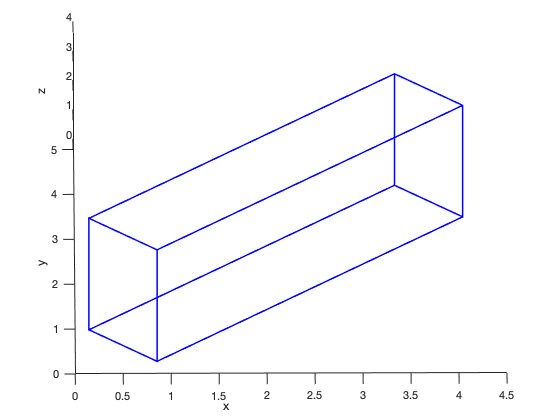
\includegraphics[width=12cm]{figures/obstacle_ex.png}
\end{figure}

\section{路径求解算法测试}
\par 关于路径求解算法的正确性测试,主要是障碍物碰撞检查算法和路径寻找算法正确性的测试,且数据为完成障碍物计算并离散到指定精度下的数据,障碍物碰撞检查算法主要是公式\ref{con:innerABandCD}和\ref{con:innerDAandBC}的应用,路径寻找算法是应用BFS或A*算法在指定精度下寻找格点路径,路径拟合算法是通过结合路径寻找算法和障碍物碰撞检测算法从而找到一条最短的路径。
数据采用上述表\ref{tab:process_input_test_data1}中关于障碍物计算算法测试的数据,首先起点P(0,0,0)到终点Q(50,50,50)的线段与障碍物的关系如图\ref{fig:insect_ex_insected},此时线段是与障碍物相交的,即不可以直接到达的情况。
\begin{figure}[htb]
    \centering
    \caption{障碍物与起点到终点线段的关系}
    \label{fig:insect_ex_insected}
    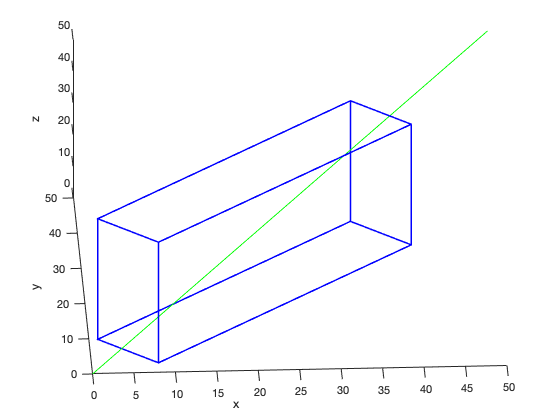
\includegraphics[width=12cm]{figures/insect_ex_insected.png}
\end{figure}
将线段$\vec{PQ}=P+k\cdot PQ=(0,0,0)+k(50-0,50-0,50-0)=(50k,50k,50k)$和障碍物代入障碍物碰撞检查算法进行测试,步骤如下:
\begin{enumerate}
    \item 初始化可行解k范围为[0,1];
    \item 对障碍物的z取值进行计算,由$k_i=\dfrac{z_i}{50k}$解得新的可行解范围[0.04,0.8];
    \item 对障碍物进行公式\ref{con:innerABandCD}检查,计算得到系数、常数分别为$a_1=0,b_1=-224,a_2=0,b_2=-224$,此时退化为一次函数,由于$b_1b_2>0$可知满足公式,此时不对k范围做更新;
    \item 对障碍物进行公式\ref{con:innerDAandBC}检查,计算得到系数、常数分别为$a_1=-700,b_1=63,a_2=700,b_2=-511$,此时$\Delta=98344960000>0$,解的新k的取值为[0.09,0.73];
    \item 综上,存在k的有效范围为[0.09,0.73],故线段PQ与障碍物相交;
\end{enumerate}
\par 对寻路算法进行测试,使用算法对该起点、终点和障碍物进行寻路操作,此时找到的拟合格点路径所经过点如图\ref{fig:find_path_ex_out}。
\begin{figure}[htb]
    \centering
    \caption{寻路算法测试输出}
    \label{fig:find_path_ex_out}
    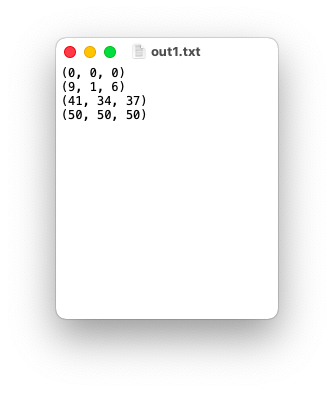
\includegraphics[width=8cm]{figures/find_path_ex_out.png}
\end{figure}
此时,根据算法输出结果,将经过格点数据和障碍物在Matlab中绘制出来,如图\ref{fig:find_path_ex_paint}。此时可知该拟合路径满足不与障碍物相交的情况下,路径长度最短的条件。
\begin{figure}[htb]
    \centering
    \caption{寻路算法测试路径与障碍物关系}
    \label{fig:find_path_ex_paint}
    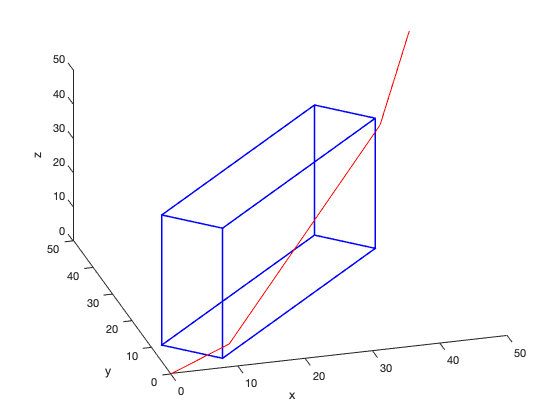
\includegraphics[width=10cm]{figures/find_path_ex_paint.png}
\end{figure}

\section{综合测试}
\par 完成对算法包含的主要模块:数据处理算法、路径求解算法的测试之后,还需要对整个算法进行全面的样例测试,需要包含多个场景,常见或稀有场景,以测试算法的稳定性。

\subsection{常见室内场景}
\par 常见室内场景,其中包含沙发、板凳、电视和冰箱等物体,根据图\ref{fig:test_common_situation_reality}中所示实际空间,建模数据为表\ref{tab:test_common_situation_data},其中包含5个障碍物。
\begin{figure}[htb]
    \centering
    \caption{常见室内空间图}
    \label{fig:test_common_situation_reality}
    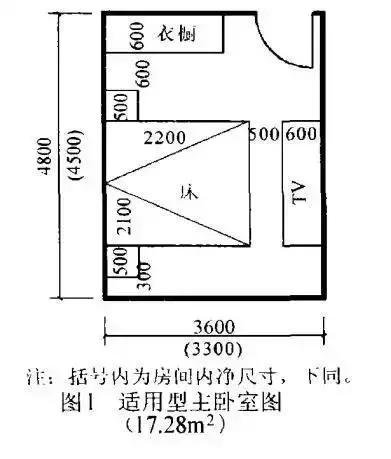
\includegraphics[width=10cm]{figures/test_common_situation_reality.JPG}
\end{figure}
\begin{table}[htb]
    \centering
    \caption{常见室内空间测试数据}
    \label{tab:test_common_situation_data}
    \begin{tabular}{cccc}
        \toprule
        起点&终点&障碍物&精度\\
        \midrule
        \multirow{5}*{(2, 0, 0)}&\multirow{5}*{(0.1, 5, 0.1)}&(0.25, 0.3), (0.25, 0.8), 0.5, [0, 0.5]&\multirow{5}*{0.1}\\
        ~&~&(1.1, 0.8), (1.1, 2.9), 2.2, [0, 0.5]&~\\
        ~&~&(0.25, 2.9), (0.25, 3.4), 0.5, [0, 0.5]&~\\
        ~&~&(0.9, 4), (0.9, 4.5), 1.8, [0, 2]&~\\
        ~&~&(3, 0.8), (3, 2.9), 0.6, [0, 1]&~\\
        \bottomrule
    \end{tabular}
\end{table}
对数据完成预处理并离散到指定精度0.1后,得到离散后数据为表\ref{tab:test_common_situation_processed_data},此时将建模后的数据在Matlab中绘制的模型俯视图和侧视图如图\ref{fig:test_common_situation_pic_top}和图\ref{fig:test_common_situation_pic_lean}。
\begin{table}[htb]
    \centering
    \caption{常见室内空间处理后数据}
    \label{tab:test_common_situation_processed_data}
    \begin{tabular}{ccc}
        \toprule
        起点&终点&障碍物\\
        \midrule
        \multirow{5}*{(20, 0, 0)}&\multirow{5}*{(1, 50, 1)}&[(0, 2), (5, 2), (5, 8), (0, 8)], [0, 5]\\
        ~&~&[(0, 8), (22, 8), (22, 28), (0, 28)], [0, 5]\\
        ~&~&[(0, 28), (5, 28), (5, 34), (0, 34)], [0, 5]\\
        ~&~&[(0, 40), (18, 40), (18, 45), (0, 45)], [0, 20]\\
        ~&~&[(27, 8), (32, 8), (32, 28), (27, 28)], [0, 10]\\
        \bottomrule
    \end{tabular}
\end{table}
\begin{figure}[htb]
    \centering
    \caption{常见室内空间处理后建模-俯视图}
    \label{fig:test_common_situation_pic_top}
    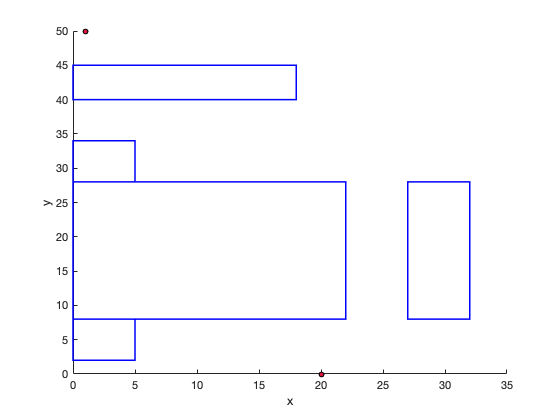
\includegraphics[width=10cm]{figures/test_common_situation_pic_top.png}
\end{figure}
\begin{figure}[htb]
    \centering
    \caption{常见室内空间处理后建模-侧视图}
    \label{fig:test_common_situation_pic_lean}
    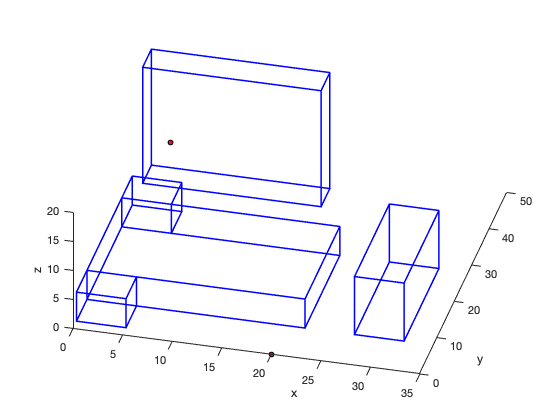
\includegraphics[width=10cm]{figures/test_common_situation_pic_lean.png}
\end{figure}
对数据进行寻路操作,设定起点为(2, 0, 0),终点为(0.1, 5, 0.1),离散在指定精度后起点为(20, 0, 0),终点为(1, 50, 1),算法得到的输出如图\ref{fig:test_common_situation_out},包含了起点、终点信息,障碍物信息以及最短路径通过的格点信息。将障碍物信息和路径信息使用Matlab绘制出来的模型的俯视图和侧视图分别如图\ref{fig:test_common_situation_out_top}和图\ref{fig:test_common_situation_out_lean},此时路径合法不经过障碍物并且满足路径长度最短。
\begin{figure}[htb]
    \centering
    \caption{常见室内空间最短路径经过顶点}
    \label{fig:test_common_situation_out}
    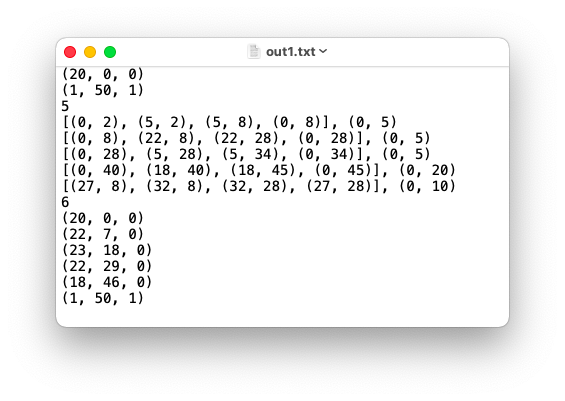
\includegraphics[width=10cm]{figures/test_common_situation_out.png}
\end{figure}
\begin{figure}[htb]
    \centering
    \caption{常见室内空间最短路径结果-俯视图}
    \label{fig:test_common_situation_out_top}
    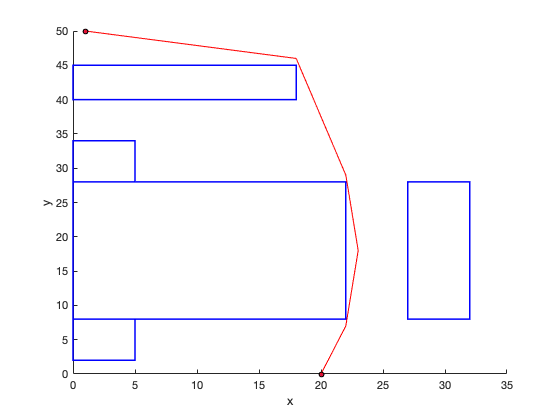
\includegraphics[width=10cm]{figures/test_common_situation_out_top.png}
\end{figure}
\begin{figure}[htb]
    \centering
    \caption{常见室内空间最短路径结果-侧视图}
    \label{fig:test_common_situation_out_lean}
    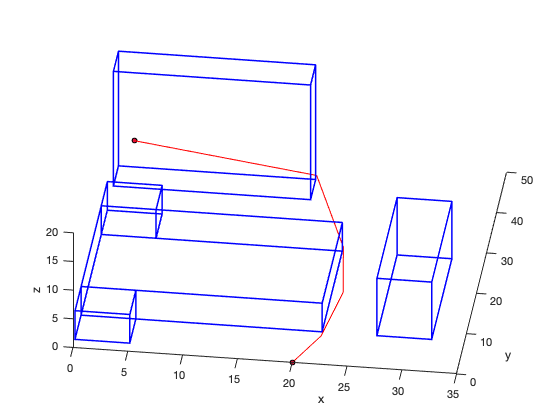
\includegraphics[width=10cm]{figures/test_common_situation_out_lean.png}
\end{figure}

\subsection{复杂室内场景}
\par 考虑在简单室内场景的基础上,增加障碍物数量和路线的复杂度,因此建模为两个房屋相邻的情况,从一个房屋到另一个房屋内的最短路径求解情况。
此时重复简单室内场景建模,原始数据为表\ref{tab:test_complex_situation_data},对其完成离散到指定精度0.1后,得到离散后的数据如表\ref{tab:test_complex_situation_processed_data},此时将处理后数据使用Matlab绘制出来可得图像的俯视图和侧视图分别为图\ref{fig:test_common_situation_processed_pic_top}和图\ref{fig:test_common_situation_processed_pic_lean}。
由建模图像可知,封闭的房屋有门和窗两处开口,此时设计出发点在左侧房间内,为(3, 0, 0),离散后为(30, 0, 0);终点在右侧房间内,为(7, 0, 0),离散后为(70, 0, 0)。所以若存在路线,应该是从左侧门进入左侧房间,通过左侧窗口离开左侧房间,再通过右侧窗口进入右侧房间,最后达到右侧门口的终点位置。使用算法在处理后的空间求出起点到终点的最短路径,此时算法输出的结果如图\ref{fig:test_complex_situation_out},其中同样包括起点、终点、障碍物信息和路径经过的顶点信息。
将输出信息使用Matlab绘制成图像,此时最短路径经过的路线图像的俯视图和侧视图分别为图\ref{fig:test_complex_situation_out_top}和图\ref{fig:test_complex_situation_out_lean},可以看出此路径满足没有经过障碍物且路径最短的条件。
\begin{table}[htb]
    \centering
    \caption{复杂室内空间测试数据}
    \label{tab:test_complex_situation_data}
    \begin{tabular}{cccc}
        \toprule
        起点&终点&障碍物&精度\\
        \midrule
        \multirow{20}*{(3, 0, 0)}&\multirow{20}*{(7, 0, 0)}&(1.35, 0), (1.35, 0.1), 2.7, [0, 2]&\multirow{20}*{0.1}\\
        ~&~&(1.65, 0), (1.65, 0.1), 3.3, [2, 2.5]&~\\
        ~&~&(0.25, 0.3), (0.25, 0.8), 0.5, [0, 0.5]&~\\
        ~&~&(3.3, 0), (3.3, 4.8), 0.1, [0, 2.5]&~\\
        ~&~&(0.05, 0), (0.05, 4.8), 0.1, [0, 2.5]&~\\
        ~&~&(1.7, 0), (1.7, 4.9), 3.3, [2.5, 2.6]&~\\
        ~&~&(1.7, 4.8), (1.7, 4.9), 3.3, [0, 2]&~\\
        ~&~&(1.9, 4.8), (1.9, 4.9), 2.8, [2, 2.5]&~\\
        ~&~&(1.1, 0.8), (1.1, 2.9), 2.2, [0, 0.5]&~\\
        ~&~&(0.25, 2.9), (0.25, 3.4), 0.5, [0, 0.5]&~\\
        ~&~&(0.9, 4), (0.9, 4.5), 1.8, [0, 2]&~\\
        ~&~&(3, 0.8), (3, 2.9), 0.6, [0, 1]&~\\
        ~&~&(5.35, 0), (5.35, 0.1), 2.7, [0, 2]&~\\
        ~&~&(5.65, 0), (5.65, 0.1), 3.3, [2, 2.5]&~\\
        ~&~&(4.25, 0.3), (4.25, 0.8), 0.5, [0, 0.5]&~\\
        ~&~&(7.3, 0), (7.3, 4.8), 0.1, [0, 2.5]&~\\
        ~&~&(4, 0), (4, 4.8), 0.1, [0, 2.5]&~\\
        ~&~&(5.7, 0), (5.7, 4.9), 3.3, [2.5, 2.6]&~\\
        ~&~&(5.7, 4.8), (5.7, 4.9), 3.3, [0, 2]&~\\
        ~&~&$\vdots$&~\\
        \bottomrule
    \end{tabular}
\end{table}
\begin{table}[htb]
    \centering
    \caption{复杂室内空间处理后测试数据}
    \label{tab:test_complex_situation_processed_data}
    \begin{tabular}{ccc}
        \toprule
        起点&终点&障碍物\\
        \midrule
        \multirow{20}*{(2, 0, 0)}&\multirow{20}*{(0.1, 5, 0.1)}&(0, 0), (27, 0), (27, 1), (0, 1), [0, 20]\\
        ~&~&(0, 0), (32, 0), (32, 1), (0, 1), [20, 25]\\
        ~&~&(0, 2), (5, 2), (5, 8), (0, 8), [0, 5]\\
        ~&~&(32, 0), (33, 0), (33, 47), (32, 47), [0, 25]\\
        ~&~&(0, 0), (1, 0), (1, 47), (0, 47), [0, 25]\\
        ~&~&(0, 0), (33, 0), (33, 49), (0, 49), [25, 26]\\
        ~&~&(0, 47), (33, 47), (33, 49), (0, 49), [0, 20]\\
        ~&~&(5, 47), (32, 47), (32, 49), (5, 49), [20, 25]\\
        ~&~&(0, 8), (22, 8), (22, 28), (0, 28), [0, 5]\\
        ~&~&(0, 28), (5, 28), (5, 34), (0, 34), [0, 5]\\
        ~&~&(0, 40), (18, 40), (18, 45), (0, 45), [0, 20]\\
        ~&~&(27, 8), (32, 8), (32, 28), (27, 28), [0, 10]\\
        ~&~&(39, 0), (66, 0), (66, 1), (39, 1), [0, 20]\\
        ~&~&(40, 0), (73, 0), (73, 1), (40, 1), [20, 25]\\
        ~&~&(40, 2), (45, 2), (45, 8), (40, 8), [0, 5]\\
        ~&~&(72, 0), (73, 0), (73, 47), (72, 47), [0, 25]\\
        ~&~&(39, 0), (40, 0), (40, 47), (39, 47), [0, 25]\\
        ~&~&(40, 0), (73, 0), (73, 49), (40, 49), [5, 26]\\
        ~&~&(40, 47), (73, 47), (73, 49), (40, 49), [0, 20]\\
        ~&~&$\vdots$\\
        \bottomrule
    \end{tabular}
\end{table}
\begin{figure}[htb]
    \centering
    \caption{常见室内空间处理后建模-俯视图}
    \label{fig:test_common_situation_processed_pic_top}
    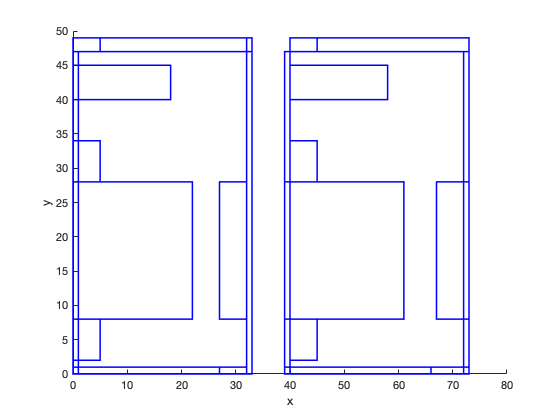
\includegraphics[width=10cm]{figures/test_complex_situation_pic_top.png}
\end{figure}
\begin{figure}[htb]
    \centering
    \caption{常见室内空间处理后建模-侧视图}
    \label{fig:test_common_situation_processed_pic_lean}
    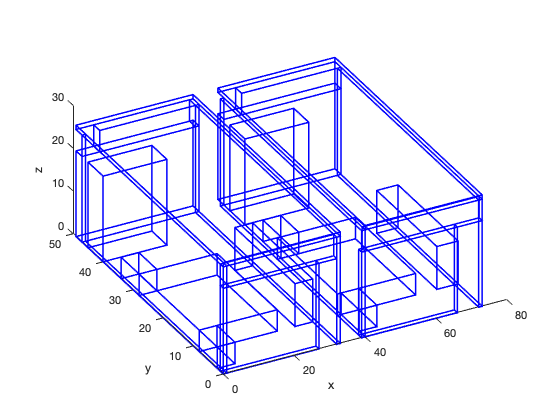
\includegraphics[width=10cm]{figures/test_complex_situation_pic_lean.png}
\end{figure}
\begin{figure}[htb]
    \centering
    \caption{复杂室内空间最短路径结果}
    \label{fig:test_complex_situation_out}
    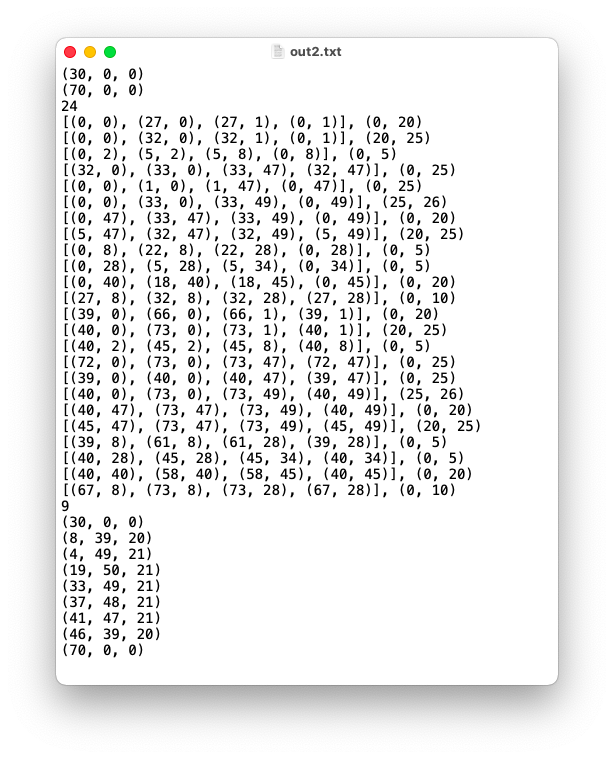
\includegraphics[width=10cm]{figures/test_complex_situation_out.png}
\end{figure}
\begin{figure}[htb]
    \centering
    \caption{复杂室内空间最短路径结果-俯视图}
    \label{fig:test_complex_situation_out_top}
    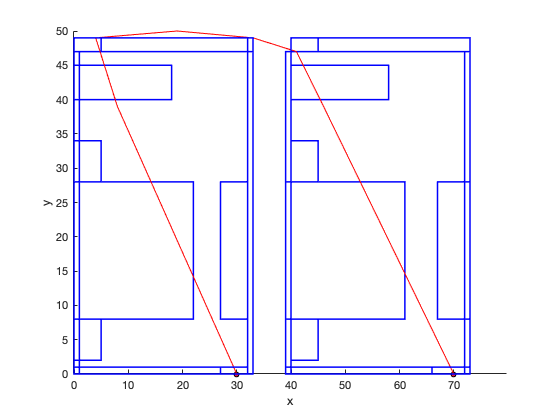
\includegraphics[width=10cm]{figures/test_complex_situation_out_top.png}
\end{figure}
\begin{figure}[htb]
    \centering
    \caption{复杂室内空间最短路径结果-侧视图}
    \label{fig:test_complex_situation_out_lean}
    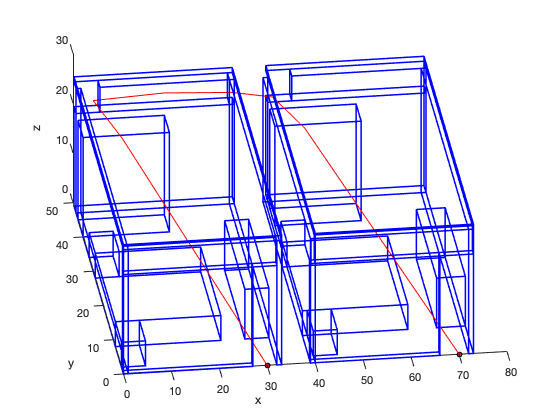
\includegraphics[width=10cm]{figures/test_complex_situation_out_lean.png}
\end{figure}

\subsection{无法到达情况}
\par 除了考虑常见的室内场景和复杂的室内场景,还需要检查算法是否能在无法到达的情况下给出无法找到路径的提示,因此在简单室内场景中将起点和终点分别置于室内和室外,并且房屋密闭不留出门窗,此时是不存在有效路径可以完成起点到终点的。
因此数据如表\ref{tab:test_cant_situation_data},数据包含10个障碍物构成的房屋场景,以及指定精度为0.1。对数据进行离散到精度0.1的操作,得到的数据为表\ref{tab:test_not_situation_processed_data},此时将处理后的障碍物数据绘制到Matlab中,可以得到的建模信息的俯视图和侧视图分别为图\ref{fig:test_not_situation_pic_top}和图\ref{fig:test_not_situation_pic_lean}。
此时使用算法求解起点(2, 1, 0),离散后为(20, 10, 0),到终点(0.1, 5, 0.1),离散后为(1, 50, 1)的最短路径,此时算法输出为图\ref{fig:test_not_situation_out},无路径信息表示未找到有效路径,符合我们设计的条件。
\begin{table}[htb]
    \centering
    \caption{无法到达情况空间测试数据}
    \label{tab:test_cant_situation_data}
    \begin{tabular}{cccc}
        \toprule
        起点&终点&障碍物&精度\\
        \midrule
        \multirow{10}*{(2, 1, 0)}&\multirow{10}*{(0.1, 5, 0.1)}&(0.25, 0.3), (0.25, 0.8), 0.5, [0, 0.5]&\multirow{10}*{0.1}\\
        ~&~&(1.1, 0.8), (1.1, 2.9), 2.2, [0, 0.5]&~\\
        ~&~&(0.25, 2.9), (0.25, 3.4), 0.5, [0, 0.5]&~\\
        ~&~&(0.9, 4), (0.9, 4.5), 1.8, [0, 2]&~\\
        ~&~&(3, 0.8), (3, 2.9), 0.6, [0, 1]&~\\
        ~&~&(1.7, 0), (1.7, 0.1), 3.3, [0, 2.5]&~\\
        ~&~&(1.7, 4.7), (1.7, 4.8), 3.3, [0, 2.5]&~\\
        ~&~&(0.05, 0), (0.05, 4.8), 0.1, [0, 2.5]&~\\
        ~&~&(3.35, 0), (3.35, 4.8), 0.1, [0, 2.5]&~\\
        ~&~&(1.7, 0), (1.7, 4.8), 3.3, [2.5, 2.6]&~\\
        \bottomrule
    \end{tabular}
\end{table}
\begin{table}[htb]
    \centering
    \caption{无法到达情况空间处理后数据}
    \label{tab:test_not_situation_processed_data}
    \begin{tabular}{ccc}
        \toprule
        起点&终点&障碍物\\
        \midrule
        \multirow{10}*{(20, 0, 0)}&\multirow{10}*{(1, 50, 1)}&(0, 2), (5, 2), (5, 8), (0, 8), [0, 5]\\
        ~&~&[(0, 8), (22, 8), (22, 28), (0, 28)], [0, 5]\\
        ~&~&[(0, 28), (5, 28), (5, 34), (0, 34)], [0, 5]\\
        ~&~&[(0, 40), (18, 40), (18, 45), (0, 45)], [0, 20]\\
        ~&~&[(27, 8), (32, 8), (32, 28), (27, 28)], [0, 10]\\
        ~&~&[(0, 0), (33, 0), (33, 1), (0, 1)], [0, 25]\\
        ~&~&[(0, 47), (33, 47), (33, 47), (0, 47)], [0, 25]\\
        ~&~&[(0, 0), (1, 0), (1, 47), (0, 47)], [0, 25]\\
        ~&~&[(33, 0), (34, 0), (34, 47), (33, 47)], [0, 25]\\
        ~&~&[(0, 0), (33, 0), (33, 47), (0, 47)], [25, 26]\\
    \end{tabular}
\end{table}
\begin{figure}[htb]
    \centering
    \caption{无法到达情况空间建模-俯视图}
    \label{fig:test_not_situation_pic_top}
    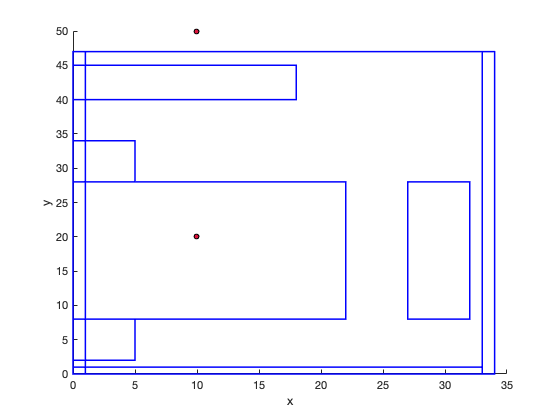
\includegraphics[width=10cm]{figures/test_not_situation_pic_top.png}
\end{figure}
\begin{figure}[htb]
    \centering
    \caption{无法到达情况空间建模-侧视图}
    \label{fig:test_not_situation_pic_lean}
    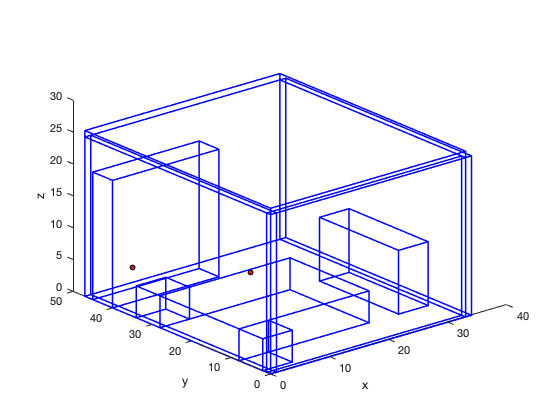
\includegraphics[width=10cm]{figures/test_not_situation_pic_lean.png}
\end{figure}
\begin{figure}[htb]
    \centering
    \caption{无法到达情况算法输出}
    \label{fig:test_not_situation_out}
    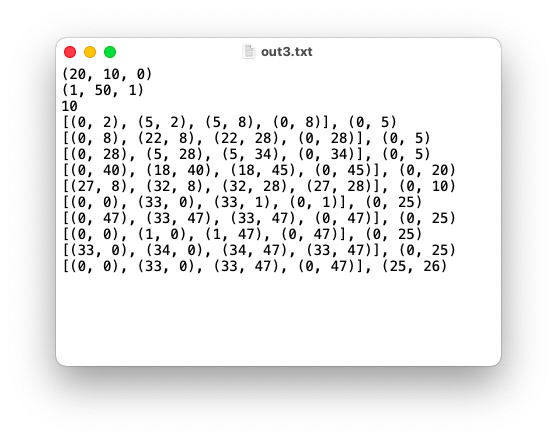
\includegraphics[width=10cm]{figures/test_not_situation_out.png}
\end{figure}

\section{本章总结}
\par{\kaishu 本章主要是对整个算法正确性进行了测试,使用了相关的测试样例和使用了Matlab绘图辅助显示。对主要模块:数据处理算法、路径求解算法进行了测试并分析,数据处理算法主要是代码\ref{code:obstacle_vertice_process}的应用,即将输入只包含底面两中点、边长和z轴范围的障碍物数据处理出底面顶点坐标信息,进而可以被后续算法使用;
路径求解算法主要测试关于使用BFS或A*算法求解起点到终点的格点路径,以及使用公式\ref{con:innerABandCD}和\ref{con:innerDAandBC}的应用以判断线段与障碍物的关系以判断是否路径可以拟合。
\par 其次是对整个算法进行综合测试,构造了常见室内场景空间、复杂场景空间以及无法到达情况空间的数据以测试算法正确性,通过分析算法输出和Matlab辅助显示判断算法是否符合预期效果。
\par 至此,整个算法已经完成构思、编码和测试的环节。}